\documentclass[dvisnames]{beamer}
% begin handouts 
%\documentclass[handout]{beamer}
%\usepackage{pgfpages}
%\pgfpagelayout{4 on 1}[a4paper,border shrink=5mm,landscape]
% end   handouts

\usepackage[utf8x]{inputenc} %Para poner acentos directamente
\usepackage{beamerthemesplit}
\usepackage{verbatim}
\usepackage{url}
 
%\usetheme{Bergen}
%\usetheme{Berlin} % se ven bien los nombres de autores
%\usetheme{Darmstadt}
\usetheme{Dresden} % se ven bien los nombres de autores
%\usetheme{Goettingen} %cosas raras, pero interesante igual
%\usetheme{Marburg} %cosas raras, pero interesante igual 
%\usetheme{Szeged}

%colores
%\definecolor{butia}{rgb}{0.45, 0.75, 0.00} 
%\usecolortheme[named=butia]{structure}
\usecolortheme[named=blue]{structure}
%\usecolortheme[named=green]{structure}
%endcolores

\title{SLAM: Simultaneous Localization And Mapping}
\author[\Tiny{Martín Llofriu \and Federico Andrade}]{Martín Llofriu \and Federico Andrade}
\institute[pgSLAM]{
\tiny{Instituto de Computación, Facultad de Ingeniería, Universidad de la República\\J. Herrera y Reissig 565, Montevideo, Uruguay\\
\href{http://www.fing.edu.uy/\~pgslam}{http://www.fing.edu.uy/~pgslam} \\
\texttt{pgslam@fing.edu.uy}
}}

\date{22/06/2011}

\begin{document}

\frame{\titlepage}

\pgfdeclareimage[height=0.5cm]{congres-logo}{imagenes/logo.png}
\pgfdeclareimage[height=0.5cm]{slam-logo}{imageness/logo.png}

\logo{\pgfuseimage{congres-logo}}

\setbeamertemplate{sidebar left}
{
\logo{\pgfuseimage{slam-logo}}
\vfill%
\rlap{\hskip0.1cm\insertlogo}%
\vskip9pt%
}
	
%\setbeamertemplate{navigation symbols}{} 
\setbeamertemplate{table of contents}{}

\section[Agenda]{}
\frame{\tableofcontents}


\setbeamertemplate{background canvas}{}

\section{Introducción}
\subsection{El problema de SLAM}
\begin{frame}
  \frametitle{SLAM: Localización y armado de mapas simultaneo}
  \begin{center}
    \begin{itemize}
	    \item Se busca resolver los problemas que plantea colocar un robot móvil en un entorno y posición desconocidos, y que el mismo sea capaz de construir incrementalmente un mapa consistente del entorno al tiempo que utiliza dicho mapa para determinar su propia localización.
	    \item<2-> Una posición precisa es necesaria para construir un mapa y un buen mapa necesario para estimar la posición. 
        \item<3-> Fundamental si se quiere aumentar la autonomía del robot para desempeñar tareas con la menor cantidad de información posible.
        \item<4-> Ha sido objeto de estudio por parte de la comunidad científica durante los últimos 20 años.        
	\end{itemize}
    \end{center}
\end{frame}


 \frame {
  \frametitle{Motivación}
  \begin{center}
	\begin{itemize}
        \item Necesidad de robots capaces de navegar de forma autónoma en terrenos inhóspitos y desconocidos por humanos.
	    \item<2-> Algunos problemas que motivan a investigadores a presentar soluciones robóticas pueden ser:
            \begin{itemize}
            \item<2-> Operaciones de búsqueda y rescate. 
            \item<2-> Exploración tanto espacial como submarina.                        
            \end{itemize}
	    \item<3-> Es un problema abierto.        
	\end{itemize}
  \end{center}
}

\frame {
  \frametitle{Dificultades}
  \begin{center}
	\begin{itemize}
	    \item Sensores (entorno y odometría)
		  \begin{itemize}
		 	   \item Ruido en las lecturas. 
			   \item Capacidades limitadas.               
		  \end{itemize}	    
		\item<2-> Cerrar ciclos
		  \begin{itemize}
		 	   \item<2-> Reconocer un lugar en el que ya estuve.
               \item<2-> Capacidad de asociar una observación con un lugar conocido.
		  \end{itemize}
		\item<3-> Lugares diferentes con idénticos valores.	
        \item<4-> Capacidad computacional
            \begin{itemize}
		 	   \item<4-> Cantidad de información creciente (memoria).
               \item<4-> Armado del mapa y actualización de posición en tiempo real (procesador). 
		    \end{itemize}	  
	\end{itemize}
  \end{center}
}

\subsection{Clasificaciones de SLAM}
\frame {
  \frametitle{Clasificación}
  \begin{itemize} 
    \item Offline vs. Online
    \begin{itemize}
		\item<2 -> Offline:Calcula la pose en base a todas las observaciones anteriores.        	
        \item<3 -> Online: Calcula la pose en base a las últimas observaciones. %a las dos últimas o a "algunas" no? supongo q lo seteas con un parámetro
    \end{itemize}	  
    \item<4 -> Topológico vs. Métrico
    \begin{itemize}
		\item<5-> Topológico: Se organizan los mapas en base a características o señales.
        \item<6-> Métricos: Se crean los mapas en base a distancias.
	\end{itemize}      
  \end{itemize}
}

\frame {
  \frametitle{Clasificación}
  \begin{itemize} 
    \item Activo vs. Pasivo
    \begin{itemize}
		\item<2 -> Activo: SLAM activo controla el movimiento del robot. Los algoritmos que implementan SLAM activo consiguen mapas mas precisos en menos tiempo.
        \item<3 -> Pasivo: En este caso el algoritmo de SLAM es puramente observador. Alguna otra entidad se encarga del control del robot. La gran mayoría de algoritmos caen dentro de esta clasificación ya que simplifica la resolución.%sospecho que teniendo el control se pueden mejorar algunas cosas
    \end{itemize}    
  \end{itemize}
}


\frame {
  \frametitle{Clasificación}
  \begin{itemize} 
    \item Estático vs. Dinámico
    \begin{itemize}
		\item<2 -> Estático: Considera que el entorno no cambia con el transcurso del tiempo. Es más utilizado ya que simplifica el problema.
        \item<3 -> Dinámico: Se acerca más a la realidad considerando ambientes cambiantes. Suelen ser más robustos que los estáticos. Se considera "las cosas que se mueven" como ruido.
	\end{itemize}
    \item<4-> Volumétrico vs. Basado en marcas
    \begin{itemize}
		\item<5-> Volumétrico: El mapa es muestreado a una muy alta resolución. Involucra un alto costo computacional.
        \item<6-> Basado en marcas: El mapa se compone de características dispersas del entorno. 
   	\end{itemize}	      
  \end{itemize}
}


\section{Estado de arte}
\subsection{SLAM en la actualidad}
\frame {
  \frametitle{Enfoques}
  \begin{itemize} 
    \item SLAM Probabilísticos    
    \item<2-> SLAM BioInspirados
  \end{itemize}
}


\subsection{SLAM Probabilísticos}

\frame {
  \frametitle{SLAM Probabilísticos}
  \begin{itemize}
	\item Introducción
	\item<2 -> Paramétricos Vs No-Paramétricos 
	\item<3 -> Técnicas de SLAM
  \begin{itemize}
	\item<4 ->Filtros de Kalman Extendidos
        \item<5 -> Filtros de Partículas
        \item<6 -> SLAM con Grafos 
  \end{itemize}
 \end{itemize}
}
\frame {
  \frametitle{Introducción}
\begin{itemize}
	  \item Usan una distribución de probabilidad para estimar la ubicación y forma del mapa
 	\begin{figure}
		 	 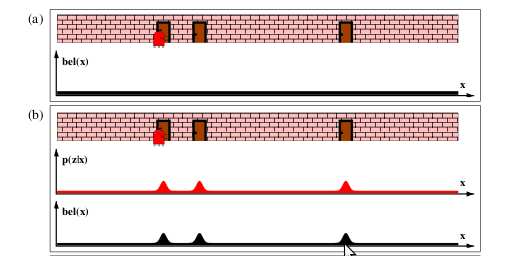
\includegraphics[scale=0.40]{imagenes/distribucion.png}
	   \end{figure}
	
  \end{itemize}
}
\frame {
  \frametitle{Introducción}
	\begin{center}
 	\begin{figure}
		 	 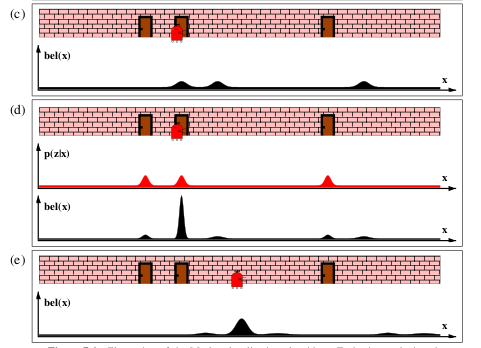
\includegraphics[scale=0.45]{imagenes/distribucion2.png}
	   \end{figure}
	\end{center}
}
\frame {
  \frametitle{Redes Bayesianas}
\begin{itemize}
	  \item Las redes bayesianas permiten representar el problema a resolver
\end{itemize}
 \begin{figure}
		 	 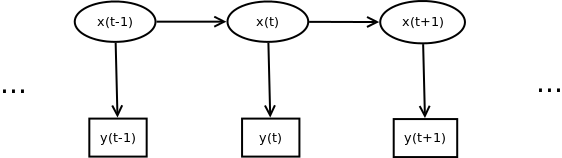
\includegraphics[scale=0.50]{imagenes/bayesKalman.png}
	   \end{figure}
}

\frame {
 \frametitle{El modelo}
  \begin{itemize}
	\item Se modela al problema de SLAM como encontrar la probabilidad 
		\\\indent\begin{math} bel(x_t) =  p(x_t|u_{1..t},z_{1..t}) \end{math}
		\\ que maximice la verosimilitud de:
		\begin{itemize}
			\item la información de odometría $u_{1..t}$
			\item la observaciones realizadas $z_{1..t}$
		\end{itemize}
 \end{itemize}
}

\frame {
  \frametitle{Filtros Bayesianos}
\begin{itemize}
	 \item<1 ->  Se basan en los filtros bayesianos 
\\\small{\begin{math} p(x_t|u_{1..t},z_{1..t}) = \frac{p(z_t | x_t, u_{1:t}) p(x_t|z_{1:t-1},u_{1:t})}{  p(z_t | z_{1:t-1}, u_{1:t}}\end{math}}
	\item<2 ->  En los métodos online actualizan esta distribución de forma continua 
		\\\small{\begin{math} bel(x_t) =  p(x_t|u_{1..t},z_{1..t}) =  \eta p(z_t|x_t) \overline{bel(x_t)}\end{math}}
		\\\small{\begin{math} \overline{bel(x_t)} =  p(x_t|u_{1..t},z_{1..t-1})=\int_{x_{t-1}}p(x_t|x_{t-1},z_{1:t-1},u_{1:t})p(x_{t-1}|z_{1:t-1},u_{1:t-1})=\int_{x_{t-1}}p(x_t|x_{t-1},z_{1:t-1},u_{1:t})bel(x_{t-1})\end{math}}
	
  \end{itemize}
}
\frame {
  \frametitle{Filtros Bayesianos}
\begin{itemize}
	\item \small{\begin{math} bel(x_t) =  \eta p(z_t|x_t) \overline{bel(x_t)}\end{math}}
	\item \small{\begin{math} \overline{bel(x_t)} =  p(x_t|u_{1..t},z_{1..t-1})=\int_{x_{t-1}}p(x_t|x_{t-1},u_{})bel(x_{t-1})\end{math}}
	 \item<1 ->  Para aplicar filtros bayesianos precisamos:
	\begin{itemize}
		\item<2-> Un modelo de odometría $p(x_t|x_{t-1}, u_t)$
		\item<3-> Un modelo de sensado $p(z_t|x_t)$
	\end{itemize}
	
  \end{itemize}
}

\frame {
  \frametitle{Ventajas y Desventajas}
\begin{itemize}
	 \item Robustos ante
		\begin{itemize}
		 \item Ruido de sensores
		\item Ruido en odometría 
		\item Errores en el modelo
		  \end{itemize}
	\item<2 ->  Representan explicitamente el concepto de incertidumbre.
	\item<3 ->  Computacionalmente costosos
	\item<4 ->  Suelen hacer aproximaciones
  \end{itemize}
}
\subsection{Paremétricos vs No Paramétricos}
\frame {
  \frametitle{Paramétricos}
\begin{itemize}
	\item<2 ->  Mantienen una representación paramétrica de la distribución de probabilidad
	\item<3 ->  Permiten una rápida actualización de la distribución de probabilidad estimada
	\item<4 ->  Asumen distribuciones conocidas, por ej. Gaussianas
  \end{itemize}
}
\frame {
  \frametitle{Paramétricos}
 \begin{figure}
		 	 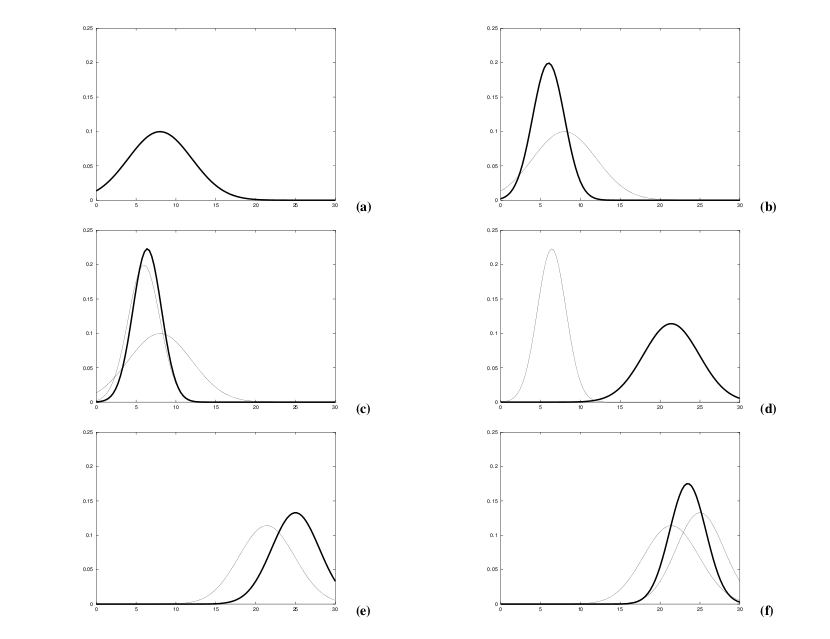
\includegraphics[scale=0.25]{imagenes/parametricos.png}
	   \end{figure}
}
\frame {
  \frametitle{No Paramétricos}
\begin{itemize}
	\item Mantienen la distribución de probabilidad representándola mediante muestras
	\item<2 ->  Pueden representar cualquier tipo de distribución
	\item<3 ->  Suelen ser más costosas computacionalmente
  \end{itemize}
}
\subsection{Técnicas de SLAM}

\frame {
  \frametitle{Filtros de Kalman}
\begin{itemize}
  	\item Asumen que la distribución de la posición del robot y de las marcas es Gaussiana
	\item<2 -> Mantiene los parámetros de moda $\mu$ y disperción $\Sigma$	
	\item<3 -> Esto permite la resolución cerrada del filtro de Bayes
  \end{itemize}
}
\frame {
  \frametitle{Filtros de Kalman}
 \begin{figure}
		 	 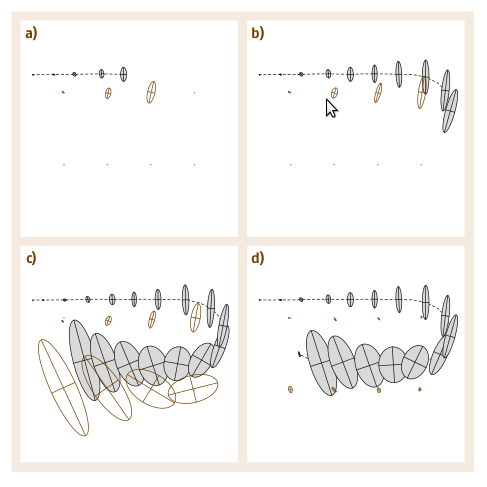
\includegraphics[scale=0.30]{imagenes/kalman.png}
	   \end{figure}
}	
\frame {
  \frametitle{Partículas}
\begin{itemize}
  	\item Mantiene partículas que representan muestras de la distribución de probabilidad
	\item<2 -> Cada partícula mantiene un estimado propio de la posición del robot y configuración del mapa
	\item<3 -> En cada iteración
	\begin{itemize}
  		\item Se actualiza la realidad de cada partícula en base a parte de la información. Usualmente se usa la información de odometría.
		\item Se le da un peso a cada partícula en función de cuanto se adapta a la información restante. Usualmente se utiliza el sensado en este paso.
		\item Se genera una nueva población de partículas tomando con reemplazo en proporción al peso asignado.
	  \end{itemize}
  \end{itemize}
}
\frame {
  \frametitle{Partículas}
 \begin{figure}
		 	 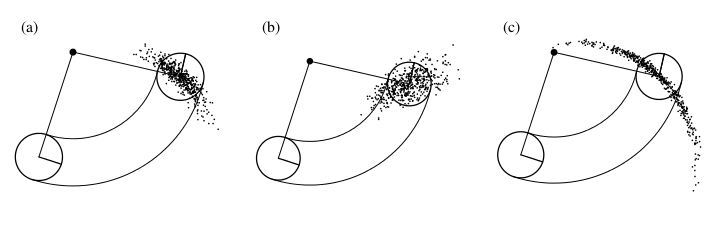
\includegraphics[scale=0.35]{imagenes/particulas.png}
	   \end{figure}
}
\frame {
  \frametitle{Partículas}
 \begin{figure}
		 	 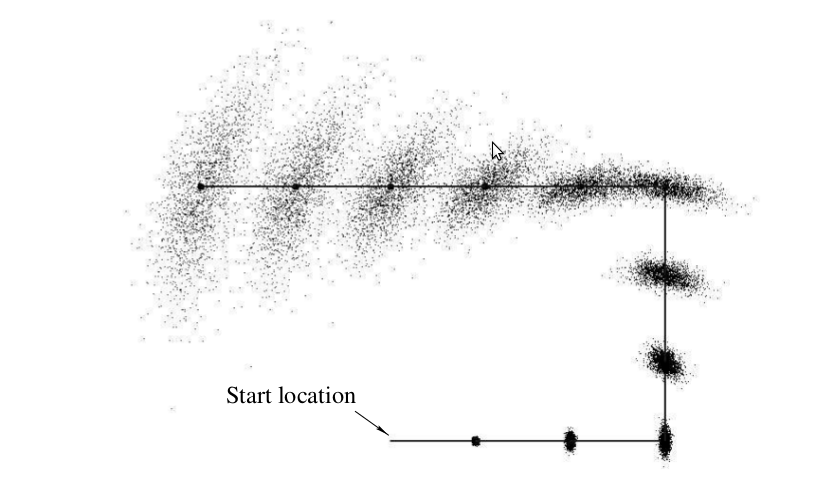
\includegraphics[scale=0.35]{imagenes/particulas2.png}
	   \end{figure}
}
\frame {
  \frametitle{SLAM con Grafos}
\begin{itemize}
  	\item Buscan llevar el problema a un problema de relajación de restricciones suaves
	\item<2 ->Construyen un grafo de restricciones en función de las medidas de odometría y sensado
	\item<3 -> Aplican un algoritmo de relajación para encontrar el camino que maximiza la verosimilitud
	\item<4 -> Suelen aplicarse a la resolución de Full SLAM
	\item<5 -> Toman ventaja de la naturaleza dispersa del grafo
  \end{itemize}
}
\frame {
  \frametitle{SLAM con Grafos}
 \begin{figure}
		 	 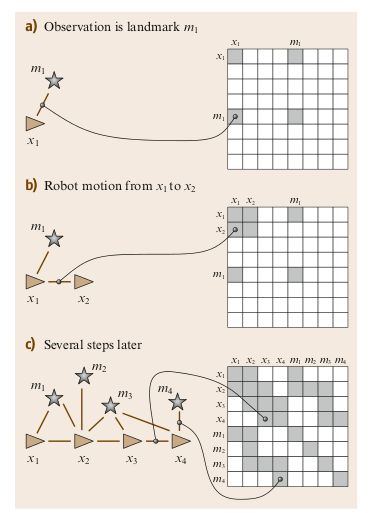
\includegraphics[scale=0.35]{imagenes/grafos.png}
	   \end{figure}
}

\subsection{SLAM BioInspirados}

\frame {
  \frametitle{RatSLAM}
  \begin{itemize} 
    \item RatSLAM    
        \begin{itemize}
		 	    \item Realiza SLAM inspirado en la naturaleza y tiempo real
                \item Los animales tienen la capacidad de almacenar y organizar señales que luego pueden usar para ubicarse.
                \item Implementan modelos simplificados del hipocampo de los roedores mediante "Redes de Atractores Continuas"(CAN).
                \item En sus últimos trabajos realizan online Slam en un barrio recorriendo una longitud de 66km. con éxito.
                %"mejorar esta oracion
                \item Utilizan solo una cámara como sensor y derivan la información de odometría de la misma.
                %el modelo de la foto parece apoyarse en odometria, no entiendo
                \item Las ratas confian en las asociaciones aprendidas entre precepciones externas y la posición estimada.
	    \end{itemize} 
  \end{itemize}
}

\frame {
  \frametitle{Rat-Slam}
%   \begin{center}
	   \begin{figure}
%			 Puertos para conectar sensores
		 	 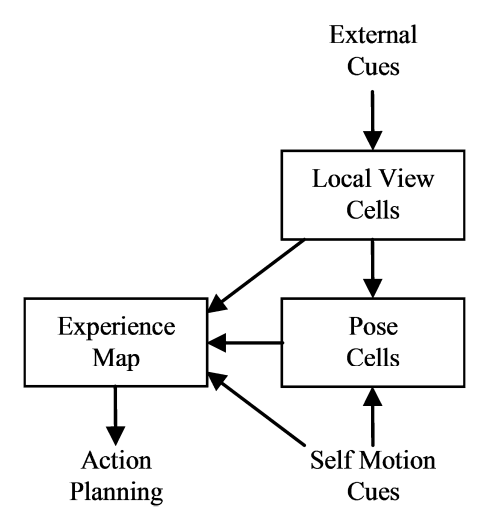
\includegraphics[scale=0.25]{imagenes/ratslamSystem.png}
	   \end{figure}
%   \end{center}  
  \begin{itemize} 
    \item Modelo utilizado en RatSLAM.        
  \end{itemize}
}


\section{Diferentes alternativas}

\subsection{Próximos pasos}
\frame {
  \frametitle{Posibles lineas de investigación}
  \begin{itemize} 
    \item Benchmarking
    \item<2-> Framework
    \item<3-> Unificación de trabajos
    \item<4-> Evaluar incluir control del robot (SLAM activo)
  \end{itemize}
}

\subsection{Benchmarking}
\frame {
  \frametitle{Estableciendo Métricas}
  \begin{itemize} 
    \item Falta en el área.    
    \item<2-> Utilizar un juego de datasets como métrica de comparación.
    \item<3-> Resultados imparciales.
    \item<4-> Extender otras propuestas existentes de benchmarking.
  \end{itemize}
}

\subsection{Framework}
\frame {
  \frametitle{Desarrollo de un entorno para SLAM}
  \begin{itemize} 
    \item Existencia de trabajos parciales
    \begin{itemize} 
        \item Permiten intercambiar modelos de sensado y odometría.
        \item Funcionan solamente con filtros de Kalman.
    \end{itemize} 
    \item<2-> SLAM a través de módulos
    \item<3-> Sirve para unificar y combinar mejoras.    	   
  \end{itemize}
}

\subsection{Unificar trabajos previos}
\frame {
  \frametitle{DP-SLAM}
  
}

\frame {
  \frametitle{DP-SLAM}
    \begin{itemize}
        \item Es un filtro de partículas.
        \item<2 -> Presenta una solución eficiente utilizando solamente un sensor láser.
        \item<3 -> Explota la independencia condicional de las celdas de ocupación propuesta por Murphy.
        \item<4 -> Evita problemas costosos de asociación de datos al no utilizar marcas.
        \item<5 -> Puede almacenar cientos de miles de posibles mapas y posiciones del robot en tiempo real.
    \end{itemize}
}

\frame {
  \frametitle{DP-SLAM}
    \begin{itemize}    
    \item Otros enfoques proponen almacenar un nuevo mapa y pose para cada partícula.
        \begin{itemize}
            \item Costo computacional muy alto (procesamiento y memoria).
            \item Complejidad \begin{math}O(MP)\end{math} (copiar el mapa).
        \end{itemize}    
    \item<2 -> DP-SLAM en lugar de asociar mapas con partículas, asocia partículas con un solo mapa y controla la cantidad de partículas.
    \item<3 -> En cada celda del mapa se almacena un árbol de partículas balanceado.
        \begin{itemize}
            \item<3 -> Contiene un historial de modificaciones de la celda.
            \item<3 -> Independiente de la cantidad de iteraciones
            \item<3 -> Complejidad \begin{math}O(ADlgP)\end{math} (M $\ll$ A).            
        \end{itemize}    
    \end{itemize}
}

\frame {
  \frametitle{DP-SLAM}
        \begin{figure}
		 	 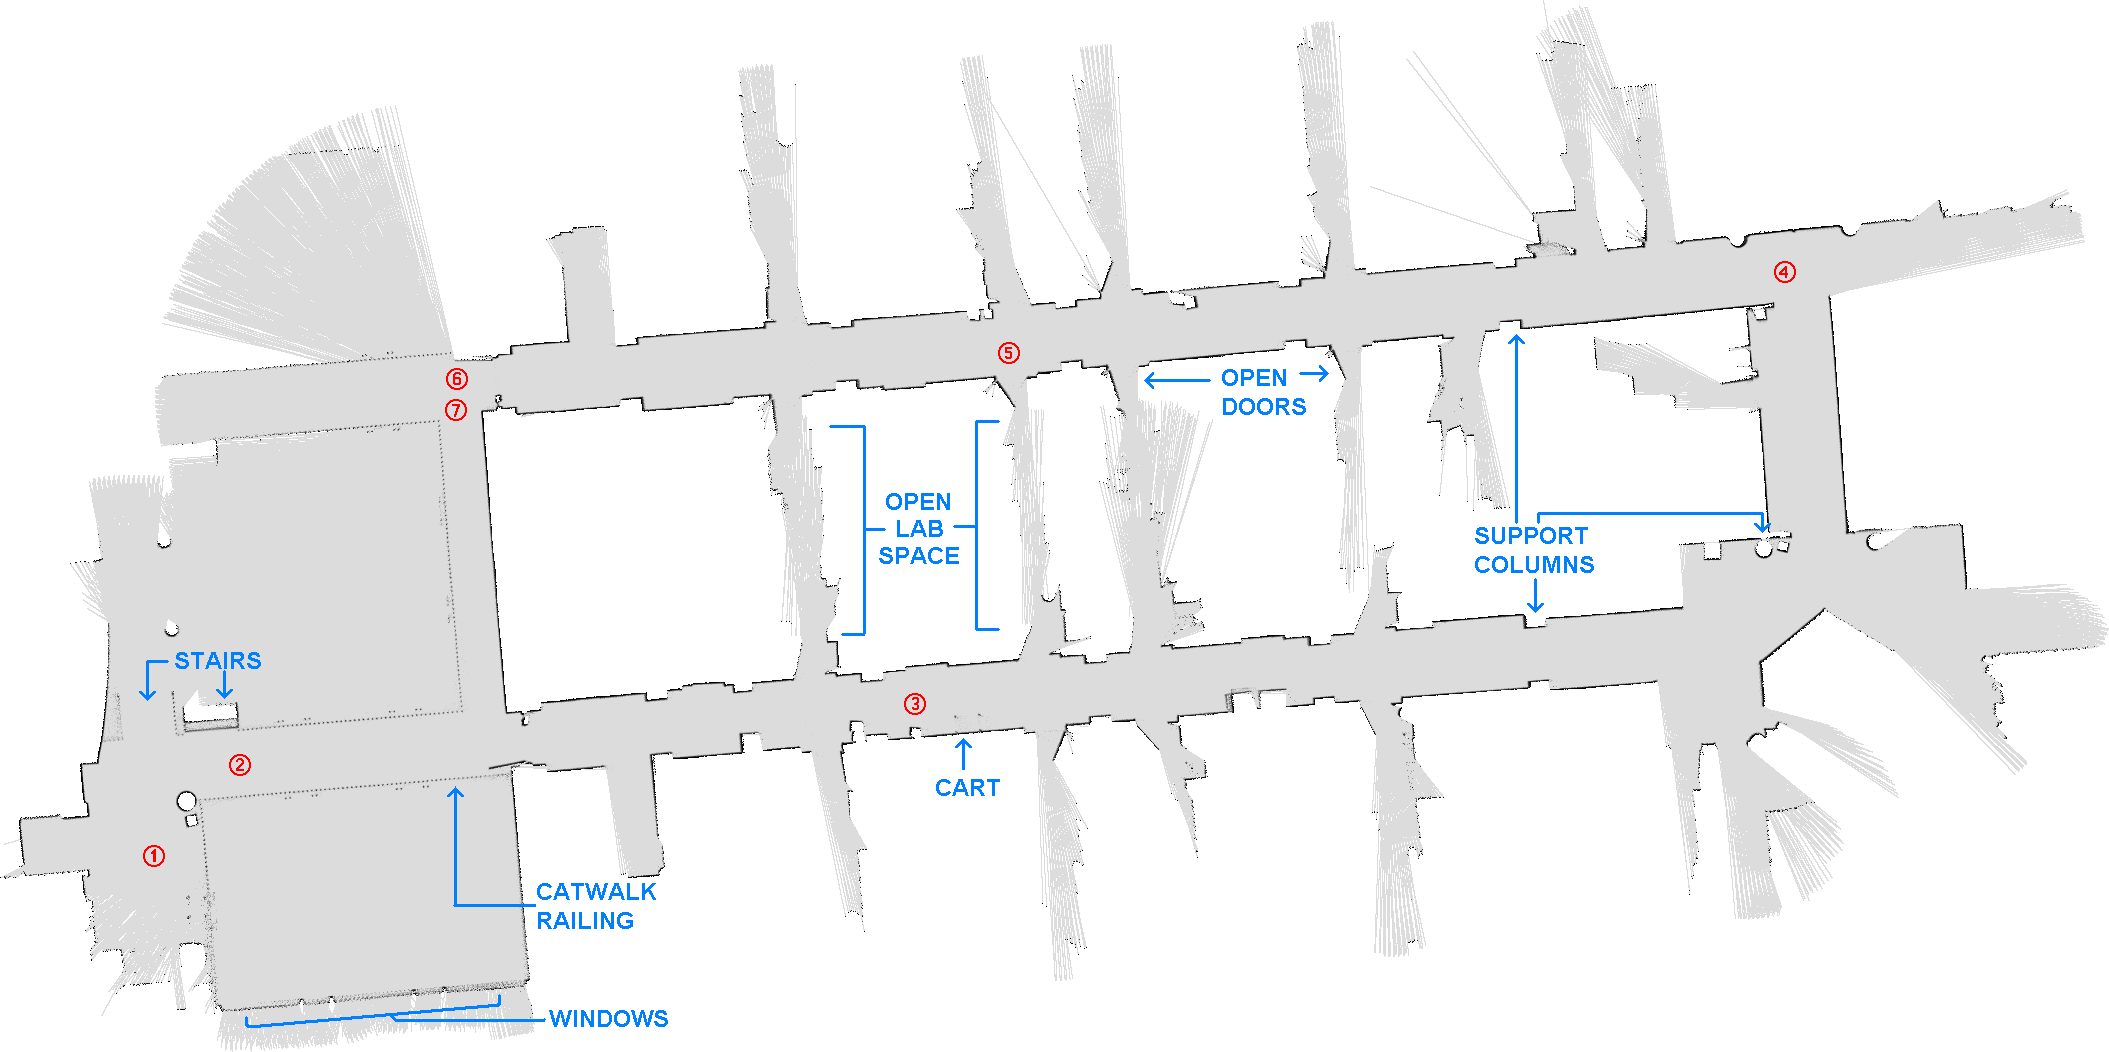
\includegraphics[scale=0.09]{imagenes/dpmapresult.png}
	    \end{figure}
    \begin{itemize}
    \item Presenta buenos resultados
        \begin{itemize}
            \item Mapas precisos (experimentalmente grillas de 3cm de lado).
            \item Cerrado de ciclos sin asunciones previas sobre el entorno.
            \item Algoritmo robusto
        \end{itemize}
    \end{itemize}
}


\frame {
  \frametitle{Grid Mapping}
    \begin{itemize}
        \item Es un filtro de partículas.
        \item<2 -> El objetivo es disminuir la cantidad de partículas necesarias.
        \item<3 -> Distribución de muestreo que considera la precisión de los sensores y toma en cuenta la última lectura del sensor.
        \item<4 -> Almacena un mapa del entorno por partícula.
        \item<5 -> Utiliza grillas (celdas de ocupación).        
    \end{itemize}
}

\frame {
  \frametitle{Grid Mapping}
    \begin{figure}
		 	 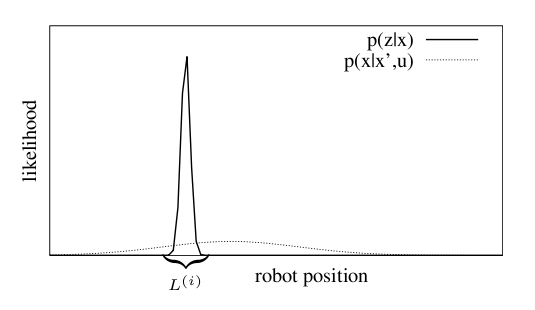
\includegraphics[scale=0.25]{imagenes/gmapping.png}
	\end{figure}
    \begin{itemize}
        \item Componentes del modelo de movimiento. El gráfico L(i) está dominado por la probabilidad de la observación realizada.
        %\item Donde creo que estoy según mi observación
        %\item Distribución de probabilidad de la posición del robot sin tener en cuenta la observación
    \end{itemize}
}

\subsection{Evaluación del control del robot}
\frame {
  \frametitle{Control sobre el SLAM}
  \begin{itemize} 
    \item No está muy estudiado en el área.
    \item<2-> Heurísticas que permitan mitigar la incertidumbre más rápidamente.
    \item<3-> SLAM como una capa de transporte confiable del robot.
  \end{itemize}
}

\appendix   

\section{Finalmente}

\subsection{Referencias}
\frame {
\frametitle{Referencias}
    \begin{itemize} 
        \item RatSLAM  - http://ratslam.itee.uq.edu.au      
        \item DP-SLAM - http://openslam.org/dpslam.html
        \item GMapping - http://openslam.org/gmapping.html
        \item Springer Handbook of Robotics
        \item Probabilistic Robotics - Sebastian Thrun
    \end{itemize}
}

\subsection{Discusión abierta}
\frame {
\frametitle{
\begin{center}
  \huge {¿Preguntas?}
\end{center}
}
}

\frame {
\frametitle{
\begin{center}
  \huge {Discusión}
    
\end{center}
}
\begin{itemize}
        \item Hacia dónde vamos?
            \begin{itemize}
                \item Benchmarking
                \item Framework
                \item Unificación de trabajos
                \item Evaluar incluir control del robot (SLAM activo)
            \end{itemize}
    \end{itemize}
}

\frame{\titlepage}

\end{document}

